\documentclass[11pt,letterpaper]{article}

% Load some basic packages that are useful to have
% and that should be part of any LaTeX installation.
%
% be able to include figures
\usepackage{graphicx}
% get nice colors
\usepackage{xcolor}

% change default font to Palatino (looks nicer!)
\usepackage[latin1]{inputenc}
\usepackage{mathpazo}
\usepackage[T1]{fontenc}
% load some useful math symbols/fonts
\usepackage{latexsym,amsfonts,amsmath,amssymb}

% comfort package to easily set margins
\usepackage[top=1in, bottom=1in, left=1in, right=1in]{geometry}

% control some spacings
%
% spacing after a paragraph
\setlength{\parskip}{.15cm}
% indentation at the top of a new paragraph
\setlength{\parindent}{0.0cm}


\begin{document}

\begin{center}
\Large
Ay190 -- Worksheet 1\\
John Pharo\\
Date: \today \\
Knights of the Realm: Anthony Alvarez, Cutter Coryell
\end{center}

\begin{figure}[!htb]\centering
  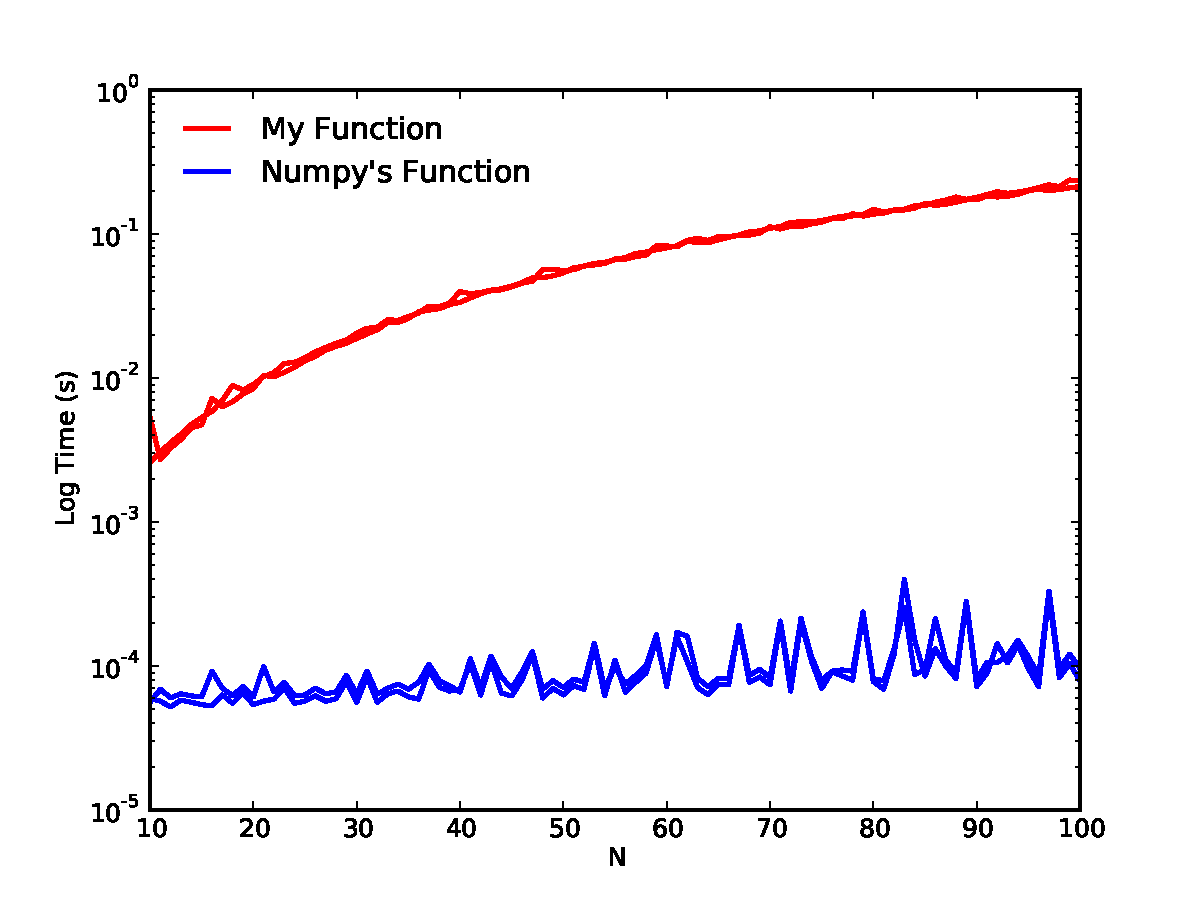
\includegraphics[width=1\textwidth]{Times}
  \caption{Plot of the time taken to compute a discrete Fourier Transform by my code and by Numpy's fft function. I'm not sure why it seems to have plotted them twice. I am also not sure why my algorithm seems to go $\propto \sqrt{N}$ instead of $\propto N^2$.}
  \end{figure}

\end{document}
